\documentclass{beamer}
\usepackage{url}
\usepackage[utf8]{inputenc}
\usepackage{comment}
\usepackage{pgf-pie}
\usepackage{multirow}
\usepackage{colortbl}
\usepackage{xcolor}
\usetheme{Madrid}
\usefonttheme{serif}
\usecolortheme{rose}

\newcommand{\keyword}{18}
\newcommand{\operadoresysimbolos}{31}
\newcommand{\literaleseidentificadores}{24}
\newcommand{\erroresyfindearchivo}{1}

\newcommand{\tokauto}{0}
\newcommand{\tokbreak}{0}
\newcommand{\tokcase}{0}
\newcommand{\tokchar}{1}
\newcommand{\tokconst}{0}
\newcommand{\tokcontinue}{0}
\newcommand{\tokdefault}{0}
\newcommand{\tokdo}{0}
\newcommand{\tokdouble}{2}
\newcommand{\tokelse}{0}
\newcommand{\tokenum}{0}
\newcommand{\tokextern}{0}
\newcommand{\tokfloat}{0}
\newcommand{\tokfor}{0}
\newcommand{\tokgoto}{0}
\newcommand{\tokif}{0}
\newcommand{\tokint}{5}
\newcommand{\toklong}{8}
\newcommand{\tokregister}{0}
\newcommand{\tokreturn}{2}
\newcommand{\tokshort}{0}
\newcommand{\toksigned}{0}
\newcommand{\toksizeof}{0}
\newcommand{\tokstatic}{0}
\newcommand{\tokstruct}{0}
\newcommand{\tokswitch}{0}
\newcommand{\toktypedef}{0}
\newcommand{\tokunion}{0}
\newcommand{\tokunsigned}{0}
\newcommand{\tokvoid}{0}
\newcommand{\tokvolatile}{0}
\newcommand{\tokwhile}{0}
\newcommand{\toklonglong}{0}
\newcommand{\toklongdouble}{0}
\newcommand{\tokbool}{0}
\newcommand{\toktrue}{0}
\newcommand{\tokfalse}{0}
\newcommand{\tokrestrict}{0}
\newcommand{\tokinline}{0}
\newcommand{\tokcomplex}{0}
\newcommand{\tokimaginary}{0}
\newcommand{\tokthreadlocal}{0}
\newcommand{\tokatomic}{0}
\newcommand{\toknoreturn}{0}

\newcommand{\tokplus}{2}
\newcommand{\tokminus}{0}
\newcommand{\tokmult}{2}
\newcommand{\tokdiv}{0}
\newcommand{\tokassign}{5}
\newcommand{\tokeq}{0}
\newcommand{\tokneq}{0}
\newcommand{\toklt}{0}
\newcommand{\tokgt}{0}
\newcommand{\tokleq}{0}
\newcommand{\tokgeq}{0}
\newcommand{\tokand}{0}
\newcommand{\tokor}{0}
\newcommand{\toknot}{0}
\newcommand{\tokbitand}{0}
\newcommand{\tokbitor}{0}
\newcommand{\tokxor}{0}
\newcommand{\tokcomplement}{0}
\newcommand{\toklshift}{0}
\newcommand{\tokrshift}{0}
\newcommand{\tokincrement}{0}
\newcommand{\tokdecrement}{0}
\newcommand{\tokdot}{0}
\newcommand{\tokarrow}{0}
\newcommand{\toklparen}{4}
\newcommand{\tokrparen}{4}
\newcommand{\toklbrace}{2}
\newcommand{\tokrbrace}{2}
\newcommand{\toklbracket}{0}
\newcommand{\tokrbracket}{0}
\newcommand{\toksemicolon}{9}
\newcommand{\tokcolon}{0}
\newcommand{\tokcomma}{1}
\newcommand{\tokellipsis}{0}

\newcommand{\tokidentifier}{18}
\newcommand{\tokintliteral}{2}
\newcommand{\tokfloatliteral}{2}
\newcommand{\tokstringliteral}{2}
\newcommand{\tokcharliteral}{0}
\newcommand{\tokboolliteral}{0}

\newcommand{\tokerror}{0}
\newcommand{\tokeof}{1}

\usepackage{listings}
\usepackage{xcolor}
\usepackage{graphicx}

\definecolor{codegreen}{rgb}{0,0.6,0}
\definecolor{codegray}{rgb}{0.5,0.5,0.5}
\definecolor{codepurple}{rgb}{0.58,0,0.82}
\definecolor{backcolour}{rgb}{0.95,0.95,0.92}

\lstdefinestyle{mycstyle}{
    language=C,
    backgroundcolor=\color{backcolour},
    moredelim=[is][\color{red}\bfseries]{|}{|},    commentstyle=\color{codegreen},
    keywordstyle=\color{magenta},
    numberstyle=\tiny\color{codegray},
    stringstyle=\color{codepurple},
    basicstyle=\ttfamily\scriptsize,
    breakatwhitespace=false,
    breaklines=true,
    captionpos=b,
    keepspaces=true,
    numbers=left,
    numbersep=5pt,
    showspaces=false,
    showstringspaces=false,
    showtabs=false,
    tabsize=2,
    frame=single
}

\title[Scaner]{Scaner}
\author[Caleb\and Sebastián \and Desireé]{Caleb Alfaro \and Sebastián Quesada \and Desireé Avilés\inst{1}}
\date[TEC 2025]{Segundo Proyecto de Compiladores, Mayo 2025}

\logo{
\includegraphics[height=0.5cm]{logoTEC.png}}

\begin{document}
\begin{frame}
  \centering
  \vspace*{0.3cm}
  
\includegraphics[scale = 0.07]{logoTEC.png}\\
  \textsc{\small Instituto Tecnológico de Costa Rica}\\[1.7em]
  \textsc{\small Compiladores e intérpretes}\\[0.3em]
  \textsc{\small Segundo Proyecto}\\[0.5em]
  \rule{\linewidth}{0.2 mm} \\[0.3 cm]
  {\LARGE \textbf{Scanner}}\\
  \rule{\linewidth}{0.2 mm} \\[0.3 cm]
  {\normalsize \emph{Caleb Alfaro, Sebastián Quesada, Desireé Avilés } }\\[1.6em]
  {\small \emph{Profesor/a:} Eddy Miguel Ramírez Jiménez}\\[0.5em]
  {\footnotesize \today}
\end{frame}

\begin{frame}{Proceso general de \textit{scanning}}
\begin{itemize}
    \item Para la etapa de preproceso se procesa el archivo fuente de forma modular, (archivo por archivo, línea por línea, char por char). Es importante destacar que en el momento en el que se procesa un  \#include, se empieza a procesar inmediatamente ese archivo, y se añade al preprocesado de salida. Esto para que no solo se mantenga el orden esperado por el usuario, sino también para que la lógica de procesos para los \#define, tenga el comportamiento esperado (que una vez definido, influya en todas las líneas por debajo de este).

    \item Los comentarios se eliminan por completo para el archivo preprocesado salida, preprocesando la línea previo al procesamiento general. Los \#defines se aplican al procesar una línea, verificando si existen apariciones y remplazando por su valor, si fuera el caso.
\end{itemize}
\end{frame}

\begin{frame}{Herramienta flex}
Flex es una herramienta generadora de analizadores léxicos, también conocidos como escáneres. Nos facilita la creación de programas que reconocen patrones léxicos en texto, utilizando expresiones regulares. Flex toma una descripción de un analizador léxico, expresada en pares de expresiones regulares y código C (reglas), y genera un archivo fuente en C que implementa el analizador.
\end{frame}

\begin{frame}{Herramienta flex}
\begin{enumerate}
 \item<1-> \textbf{Definición de reglas:} El usuario define un conjunto de reglas, donde cada regla consiste en una expresión regular y una acción en C. La expresión regular describe el patrón a buscar en el texto de entrada, y la acción en C especifica qué hacer cuando se encuentra ese patrón.
 \item<2-> \textbf{Generación de código C:} Flex toma estas reglas y genera un archivo fuente en C que contiene la implementación del analizador léxico. Este archivo contiene la lógica para encontrar y procesar los patrones definidos en las reglas.
 \item<3> \textbf{Compilación y uso:} El archivo fuente en C generado por Flex se compila con un compilador de C y se utiliza para crear un programa que realiza la tarea de analizar léxicamente el texto de entrada.
\end{enumerate}
\end{frame}

\begin{frame}[fragile]{Programa después del preproceso}{}

  \begin{lstlisting}[style=mycstyle]
int holaAndamosTesting(long long xd);
long long largo(long long grueso);
int mokeyplus(int a, int b) {
a+=b;
return a + b; 
}#errortoken nosirve
int main() {
double numPi = 3.1416;
double dosPi = 3.1416 * 2;
long long mesi= "testmessi"; 
char* mesi2 = "testmessi2"; 
return 0;
}  \end{lstlisting}
\end{frame}

\begin{frame}{Histograma de las cantidades de tokens}
\begin{table}
\begin{tabular}{p{5cm}|>{\centering\arraybackslash}p{3cm}}
         \rowcolor{blue!30}&\\
         \rowcolor{blue!30} \centering{\large \textbf{Categoría Léxica}} &  {\large \textbf{Cantidad}}\\
         \rowcolor{blue!30}&\\
         \arrayrulecolor{blue!30}
         \hline
         Palabras Reservadas & \keyword\\
         \hline
         Operadores y símbolos  & \operadoresysimbolos\\
         \hline
         Literales e identificadores &\literaleseidentificadores \\
         \hline
         Errores y fin de archivo &\erroresyfindearchivo\\
         \hline
         \end{tabular}
\end{table}
\end{frame}

\begin{frame}{Cantidades de palabras reservadas}
\begin{table}[h]
\centering
\begin{tabular}{p{2cm}|>{\centering\arraybackslash}p{1.6cm}
                |p{2cm}|>{\centering\arraybackslash}p{1.6cm}}
         \arrayrulecolor{blue!30}
        \rowcolor{blue!30} &&&\\
         \rowcolor{blue!30} 
                \centering{\textbf{Palabra}} &  
                { \textbf{Cantidad}} &
                \centering{\textbf{Palabra}} &  
                { \textbf{Cantidad}} \\
        \rowcolor{blue!30} &&&\\
        \hline
        break & \tokbreak & case & \tokcase\\
        \hline
        \rowcolor{blue!3} char & \tokchar & const & \tokconst\\
        \hline
        continue & \tokcontinue & default & \tokdefault\\
        \hline
        \rowcolor{blue!3} do & \tokdo & double & \tokdouble\\
        \hline
        else & \tokelse & enum & \tokenum\\
        \hline
        \rowcolor{blue!3} extern & \tokextern & float & \tokfloat\\
        \hline
        for & \tokfor & goto & \tokgoto\\
        \hline
        \rowcolor{blue!3} if & \tokif & int & \tokint\\
        \hline
        long & \toklong & register & \tokregister\\
        \hline
        \rowcolor{blue!3} return & \tokreturn & short & \tokshort\\
        \hline
        signed & \toksigned & sizeof & \toksizeof\\
        \hline
        \rowcolor{blue!3} static & \tokstatic & struct & \tokstruct\\
        \hline
\end{tabular}
\end{table}
\end{frame}

\begin{frame}{Cantidades de palabras reservadas}
\begin{table}[h]
\centering
\begin{tabular}{p{2cm}|>{\centering\arraybackslash}p{1.6cm}
                |p{2cm}|>{\centering\arraybackslash}p{1.6cm}}
         \arrayrulecolor{blue!30}
        \rowcolor{blue!30} &&&\\
         \rowcolor{blue!30} 
                \centering{\textbf{Palabra}} &  
                { \textbf{Cantidad}} &
                \centering{\textbf{Palabra}} &  
                { \textbf{Cantidad}} \\
        \rowcolor{blue!30} &&&\\
        \hline        
        switch & \tokswitch & typedef & \toktypedef\\
        \hline
        \rowcolor{blue!3} union & \tokunion & unsigned & \tokunsigned\\
        \hline
        void & \tokvoid & volatile & \tokvolatile\\
        \hline
        \rowcolor{blue!3} while & \tokwhile & long long & \toklonglong\\
        \hline
        long double & \toklongdouble & bool & \tokbool\\
        \hline
        \rowcolor{blue!3} true & \toktrue & false & \tokfalse\\
        \hline
        restrict & \tokrestrict & inline & \tokinline\\
        \hline
        \rowcolor{blue!3} complex & \tokcomplex & imaginary & \tokimaginary\\
        \hline
        thread\_local & \tokthreadlocal & atomic & \tokatomic\\
        \hline
        \rowcolor{blue!3} noreturn & \toknoreturn & & \\
        \hline
\end{tabular}
\end{table}
\end{frame}

\begin{frame}{Cantidades de los operadores y símbolos}
\begin{table}[h]
\centering
\begin{tabular}{p{2cm}|>{\centering\arraybackslash}p{1.6cm}
                |p{2cm}|>{\centering\arraybackslash}p{1.6cm}}
         \arrayrulecolor{blue!30}
        \rowcolor{blue!30} &&&\\
         \rowcolor{blue!30} 
                \centering{\textbf{Palabra}} &  
                { \textbf{Cantidad}} &
                \centering{\textbf{Palabra}} &  
                { \textbf{Cantidad}} \\
        \rowcolor{blue!30} &&&\\
        \hline
        plus & \tokplus & minus & \tokminus\\
        \hline
        \rowcolor{blue!3} mult & \tokmult & div & \tokdiv\\
        \hline
        assign & \tokassign & eq & \tokeq\\
        \hline
        \rowcolor{blue!3} neq & \tokneq & lt & \toklt\\
        \hline
        gt & \tokgt & leq & \tokleq\\
        \hline
        \rowcolor{blue!3} geq & \tokgeq & and & \tokand\\
        \hline
        or & \tokor & not & \toknot\\
        \hline
        \rowcolor{blue!3} bitand & \tokbitand & bitor & \tokbitor\\
        \hline
        xor & \tokxor & complement & \tokcomplement\\
        \hline
\end{tabular}
\end{table}
\end{frame}

\begin{frame}{Cantidades de los operadores y símbolos}
\begin{table}[h]
\centering
\begin{tabular}{p{2cm}|>{\centering\arraybackslash}p{1.6cm}
                |p{2cm}|>{\centering\arraybackslash}p{1.6cm}}
         \arrayrulecolor{blue!30}
        \rowcolor{blue!30} &&&\\
         \rowcolor{blue!30} 
                \centering{\textbf{Palabra}} &  
                { \textbf{Cantidad}} &
                \centering{\textbf{Palabra}} &  
                { \textbf{Cantidad}} \\
        \rowcolor{blue!30} &&&\\
        \hline  
        \rowcolor{blue!3} lshift & \toklshift & rshift & \tokrshift\\
        \hline
        increment & \tokincrement & decrement & \tokdecrement\\
        \hline
        \rowcolor{blue!3} dot & \tokdot & arrow & \tokarrow\\
        \hline
        lparen & \toklparen & rparen & \tokrparen\\
        \hline
        \rowcolor{blue!3} lbrace & \toklbrace & rbrace & \tokrbrace\\
        \hline
        lbracket & \toklbracket & rbracket & \tokrbracket\\
        \hline
        \rowcolor{blue!3} semicolon & \toksemicolon & colon & \tokcolon\\
        \hline
        comma & \tokcomma & ellipsis & \tokellipsis\\
        \hline
\end{tabular}
\end{table}
\end{frame}

\begin{frame}{Cantidades de literales e identificadores, errores y final de archivo}
\begin{table}[h]
\centering
\begin{tabular}{p{3cm}|>{\centering\arraybackslash}p{1.8cm}}
         \arrayrulecolor{blue!30}
        \rowcolor{blue!30} &\\
         \rowcolor{blue!30} 
                \centering{\textbf{Palabra}} &  
                { \textbf{Cantidad}}\\
        \rowcolor{blue!30} &\\
        identifier & \tokidentifier\\
        \hline
        \rowcolor{blue!3}intliteral & \tokintliteral\\
        \hline
        floatliteral & \tokfloatliteral\\
        \hline
        \rowcolor{blue!3}stringliteral & \tokstringliteral\\
        \hline
        error & \tokerror\\
        \hline
        \rowcolor{blue!3}eof & \tokeof\\
        \hline
         char literal &\tokcharliteral \\
        \hline
        \rowcolor{blue!3} bool literal & \tokboolliteral\\
        \hline
\end{tabular}
\end{table}
\end{frame}

\begin{frame}{Grafico de pastel}{Cantidad de cada categoría léxica}
\centering
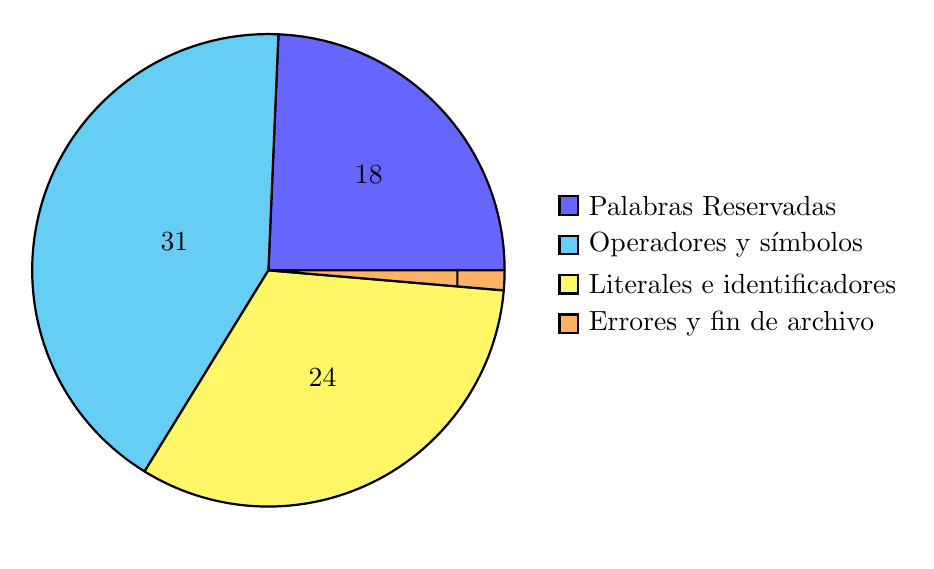
\begin{tikzpicture}
    \pie[
        sum=auto,
        text=legend
    ]
    {\keyword/Palabras Reservadas, \operadoresysimbolos/Operadores y símbolos, \literaleseidentificadores/Literales e identificadores, \erroresyfindearchivo/Errores y fin de archivo}
\end{tikzpicture}
\end{frame}

\begin{frame}{Bibliografía y fuentes consultadas}
\begin{thebibliography}{9}

\bibitem{introflexbison}
Universidad de Zaragoza. (2003-2004). \emph{Introducción a Flex y Bison}. Departamento de Informática e Ingeniería de Sistemas. \\
\url{https://webdiis.unizar.es/asignaturas/LGA/material_2003_2004/Intro_Flex_Bison.pdf}

\bibitem{mitflex}
Free Software Foundation. (s.f.). \emph{Flex: The Fast Lexical Analyzer}. Massachusetts Institute of Technology. (Trabajo original en inglés, traducido al español). \\
\url{https://web-mit-edu.translate.goog/gnu/doc/html/flex_1.html?_x_tr_sl=en&_x_tr_tl=es&_x_tr_hl=es&_x_tr_pto=sge}

\end{thebibliography}
\end{frame}

\end{document}
